\section{Results} \label{results}

\subsection{The genotype-phenotype map transforms basins of attraction}

 Initially focusing on the role of the genotype-phenotype map, we first look at the influence of the supply of heritable variation on populations evolving on a set of simple adaptive landscapes. We consider populations characterized by two loci $\alpha_1$ and $\alpha_2$ and two heritable phenotypic traits $x_1$ and $x_2$ under a set of different linear genotype-phenotype maps. Individuals are diploid, carrying two alleles per locus. The genotypic value at locus $i$ is given by $\alpha_i=\alpha_{i,1} +\alpha_{i,2}$, where $\alpha_{i,1}$ and $\alpha_{i,2}$ denote the allelic values. Mutations are introduced each generation at a per-allele mutation rate $\mu=0.025$, with mutational effects drawn from a distribution with standard deviation $\sigma=0.05$. We ran simulations for populations consisting of 1,000 diploid individuals, split evenly between males and females, over a number of discrete generations until a local fitness optimum was reached. The simulation code and analysis is deposited on Zenodo \parencite{christophnetz_2026_19204638}.
 
 We consider a linear genotype-phenotype mapping $\boldsymbol{x}=\mathbf{B}\boldsymbol{\alpha}$ \parencite{wagner1989multivariate, wagner1984eigenvalue}, and explore three different maps,  \( \mathbf{B}_1= [1, 0,  0,  1]  \), \( \mathbf{B}_2= [\frac{5}{3}, \frac{4}{3}, \frac{4}{3}, \frac{5}{3}]  \) and \( \mathbf{B}_3=[ \frac{5}{3},  -\frac{4}{3}, -\frac{4}{3}, \frac{5}{3}] \). $\mathbf{B}_1$ represents a one-to-one genotype-phenotype map, $\mathbf{B}_2$ and $\mathbf{B}_3$ lead to a distortion of the phenotypic effect of genetic variation.

 For these linear genotype-phenotype maps, the M-matrix is given by $\mathbf{M}=\Sigma \mathbf{BB}^\top$, with \( \Sigma=2\mu[ \sigma^2,  0, 0, \sigma^2] \), and is constant over phenotype space. The M-matrix under $\mathbf{B}_1$ is unbiased and has equal variance terms in both phenotypic dimensions, while under $\mathbf{B}_2$ and $\mathbf{B}_3$ the M-matrices become eccentric with positive and negative covariance terms, respectively (\FIG[]{fig1}). All three M-matrices have the same determinant and therefore cover the same volume in phenotype space over which mutations spread out. 
 
 We first look at the evolution on an adaptive landscape with a single global optimum, generated from a gaussian fitness function \FIG[A]{fig1}. 
 %$f(x_1, x_2)=e^{-\frac{(x-5.5)^2+(y-5.5)^2}{2*3^2}}$
Populations were initialized at four different locations in phenotype space away from the evolutionary optimum. As expected, populations with an unbiased M-matrix roughly follow the lines of steepest ascent, whereas populations with eccentric M-matrices are initially biased towards the direction of the dominant eigenvector of the M-matrix ('genetic lines of least resistance', \cite{Schluter1996-uo}).  

We then generated adaptive landscapes with two or more adaptive optima using Perlin noise \parencite{perlin1985image}, normalized to values between 0 and 1. Perlin noise allows the generation of landscapes with smooth variation that at the same time are computationally efficient (\nameref{methods}). The landscape we consider in \FIG[B, C\&D]{fig1} (Perlin frequency 0.15, seed 96) contains two alternative optima in the region $x_1 \in [0, 10], x_2 \in [0, 7]$, located near $(1.69, 2.96)$ and $(9.31, 3.70)$.  We observe that the genotype-phenotype map exerts a strong influence on evolutionary outcomes. Populations were initialized from a $31 \times 31$ grid of starting points spread out over $x_1 \in [2, 8], x_2 \in [0, 6]$, with 10 replicate simulation runs for each point. We focus on evolutionary outcomes, connecting each starting point to the optimum that the population converges upon. The separatrix between the basins of attraction of adjacent evolutionary optima was inferred with support vector machines (SVM, see \nameref{methods}) and is drawn as a line across the adaptive landscape, alongside the deterministic separatrix predicted by the Lande equation. We observe that developmental bias leads to a significant distortion of the basins of attraction. While the separatrix for the unbiased M-matrix runs nearly vertically down the adaptive landscape (function of the selected adaptive landscape, \FIG[B]{fig1}), it is rotated into the direction of the leading eigenvector once the M-matrix becomes biased (\FIG[C\&D]{fig1}). Thus, the M-matrix alters the evolutionary dynamics, and populations that differ in $\mathbf{M}$ can evolve from the same origin to different local optima. 

 Thus far, we have assumed linear genotype-phenotype maps where the effect of genetic variation is constant over phenotype space. In reality, the underlying developmental system determines how genetic variation is expressed at the phenotypic level and thus may change over the space of possible phenotypes. In the following, we explore how a set of simple gene regulatory motifs influences the M-matrix across phenotype space, and what effect this has for evolutionary outcomes on adaptive landscapes of varying complexity.

\begin{figure}
    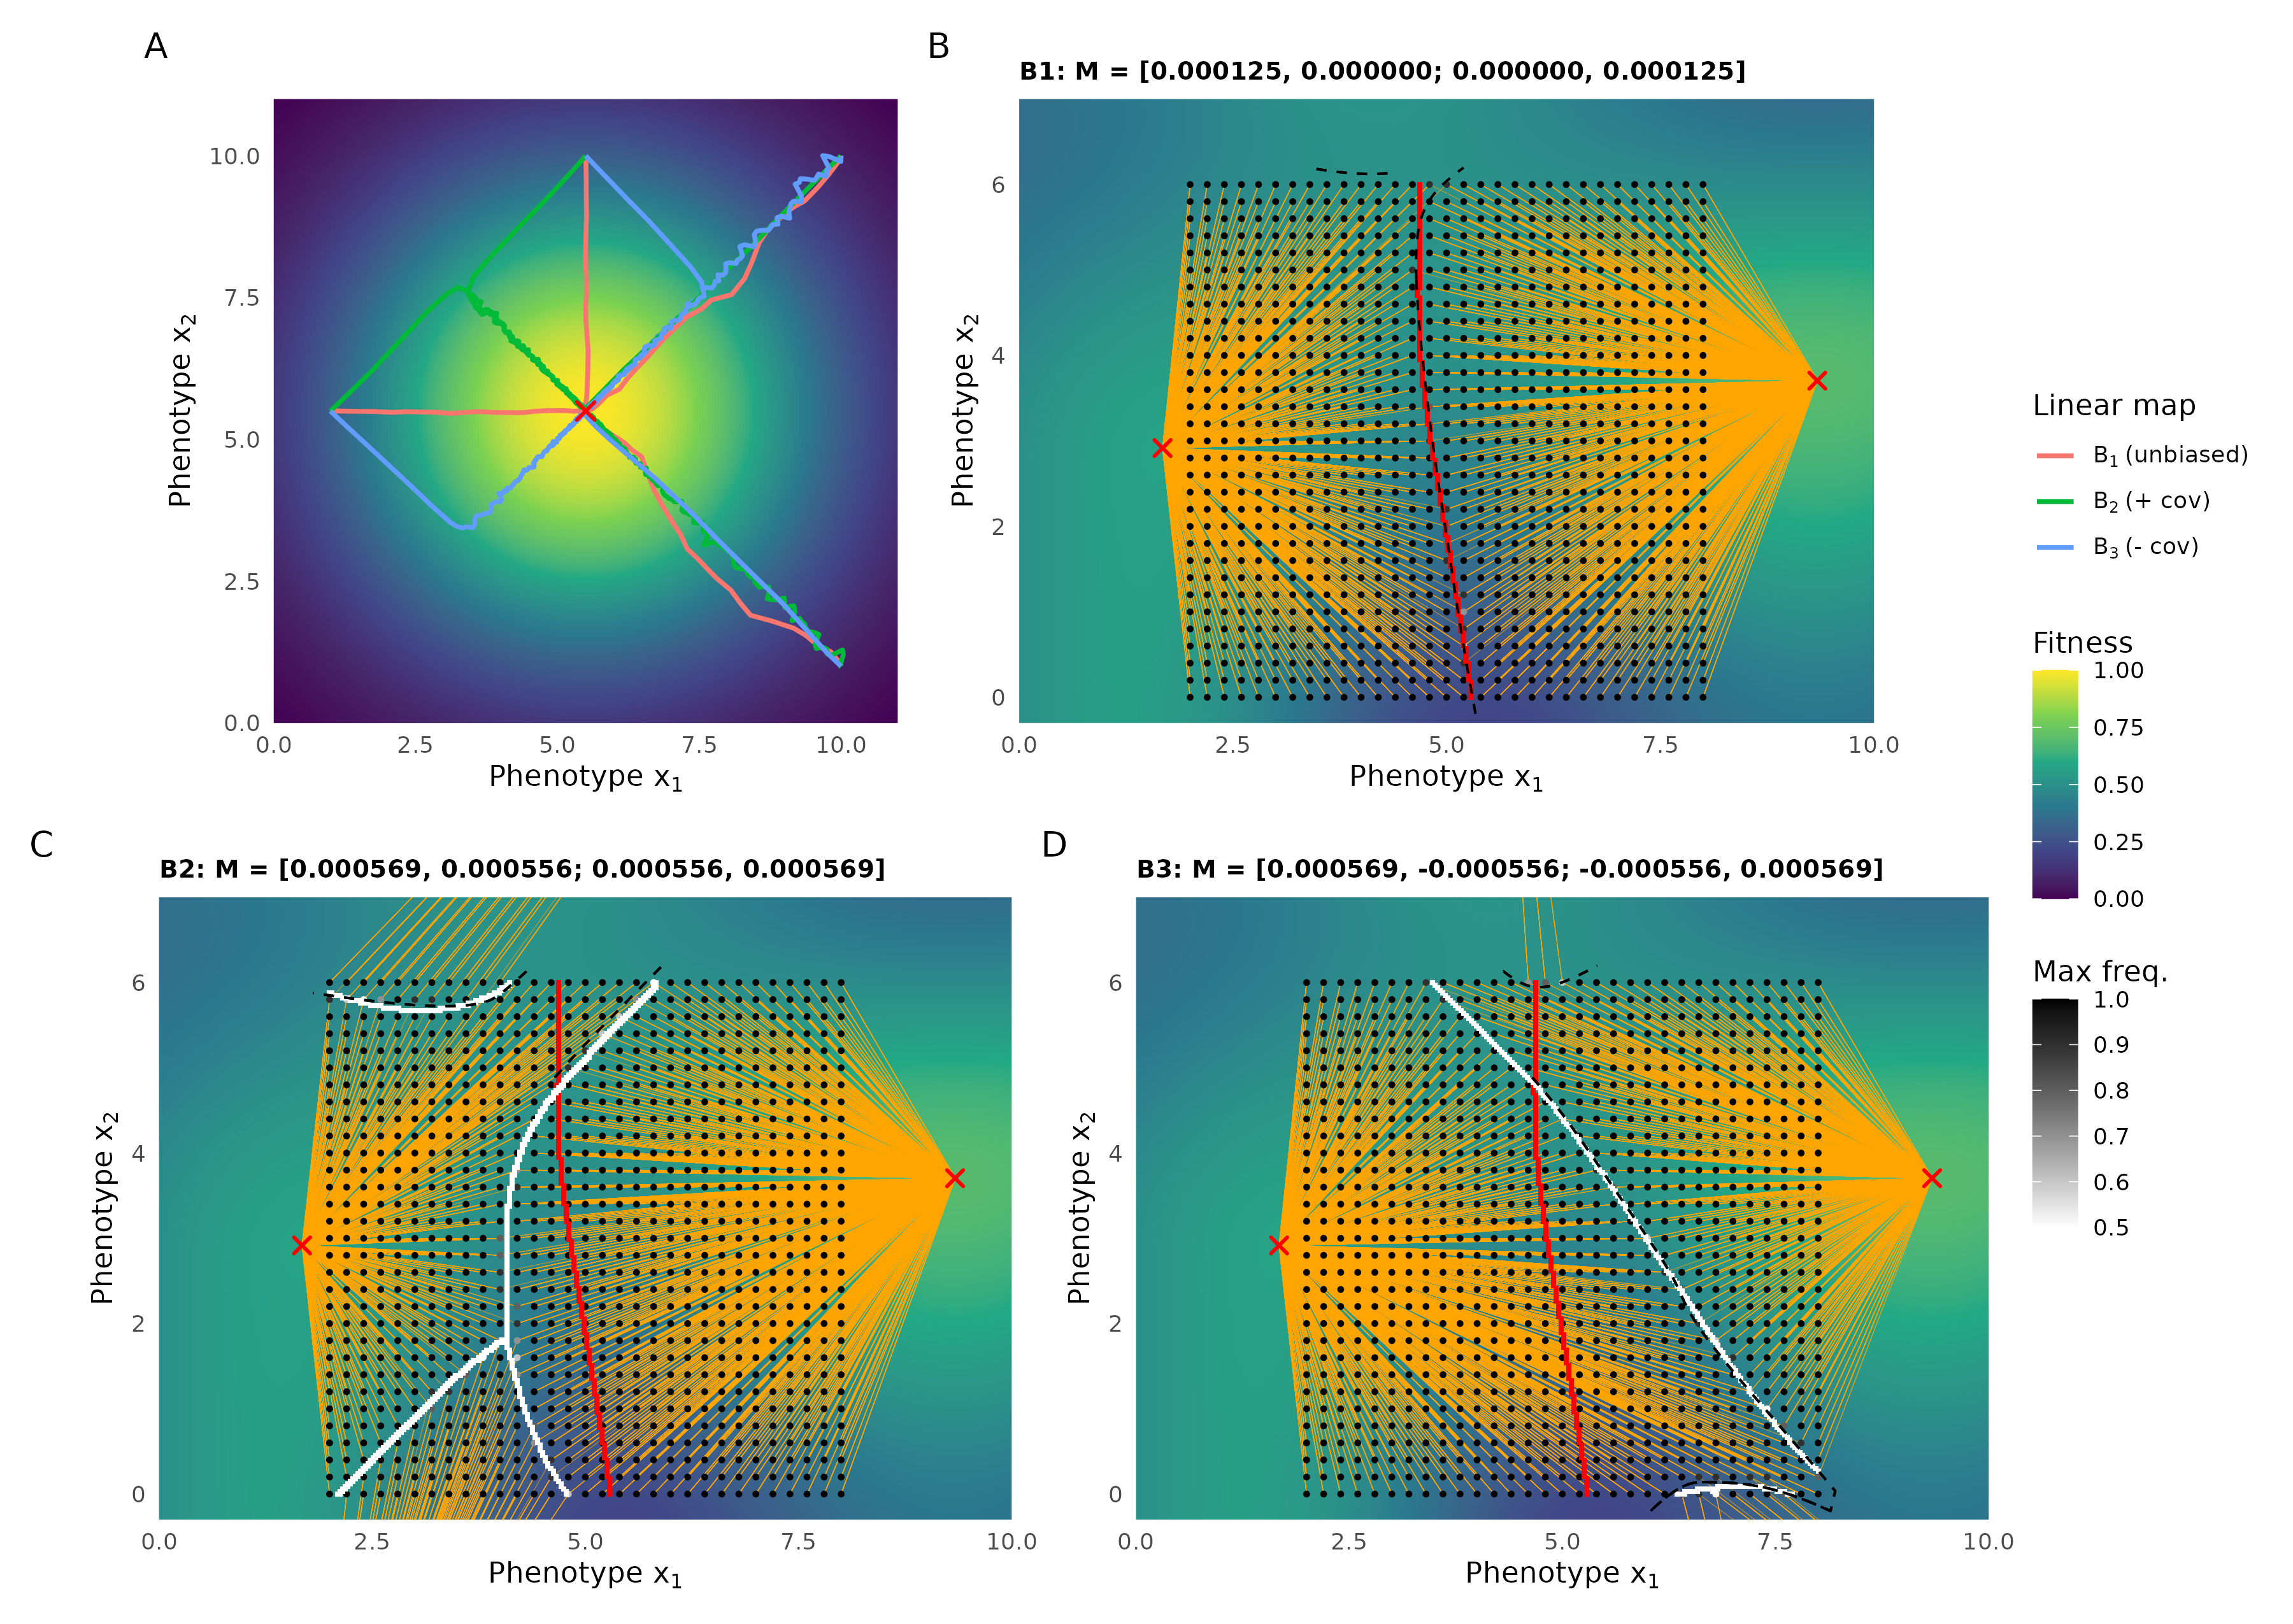
\includegraphics[width=\linewidth]{src/figures/fig1.png}
    \caption{\textbf{The effect of different linear genotype-phenotype maps on evolutionary trajectories and outcomes (A) }  In a single-peaked adaptive landscape, the shape of the M-matrix initially biases evolutionary trajectories in the direction of the dominant eigenvector. All populations converge on the same unique optimum, independently of their M-matrix. \textbf{(B, C, D)} Evolutionary simulations from a $31 \times 31$ grid of starting points, evenly spread over $x_1 \in [2, 8], x_2 \in [0, 6]$, with 10 diploid sexual replicate simulations for each point of origin (Perlin frequency 0.15, seed 96, offset $(0, -2.5)$). Each point is connected by orange edges to the optima that populations converged upon. Points are colored with respect to the frequency of the most common evolutionary outcome, such that regions where populations can evolve to multiple evolutionary optima are visible in shades of gray and white. The separatrix dividing regions of alternative evolutionary outcomes inferred by SVM is shown as a red (unbiased M-matrix, overlaid on all panels for comparison) or white (eccentric M-matrices) line; dashed black lines show the deterministic Lande-equation separatrices. The 10-fold cross-validated classification accuracy of the SVM was 99.6\%, 99.0\%, and 99.1\% for $\mathbf{B}_1$, $\mathbf{B}_2$, and $\mathbf{B}_3$, respectively. \textbf{(B)} Unbiased M-matrix without covariance ($\mathbf{B}_1$). \textbf{(C)} M-matrix with positive covariance terms ($\mathbf{B}_2$). \textbf{(D)} M-matrix with negative covariance terms ($\mathbf{B}_3$). All three M-matrices shown have the same determinant ($\mu=0.025, \sigma=0.05$, diploid). Phenotypic optima are marked in red. M-matrix entries are rounded to the 6th decimal.}
   
    \label{fig:fig1}
\end{figure}


\subsection{Gene regulation shapes phenotypic variation}

As before, we consider a set of two traits $x_1$ and $x_2$, which however are now under the control of gene regulatory networks \parencite{gjuvsland2007statistical}. These networks consist of interacting transcription factors that regulate each other’s expression. The resulting dynamics determine stable patterns of gene expression, which constitute the phenotypes. Although kept deliberately simple, these GRNs capture core features of developmental processes that dynamically generate the phenotype through developmental time \parencite{lewontin1983organism, alberch1991genes, milocco2024utilizing}. This represents a minimal developmental map between genotype and phenotype where the genotype consists of the strengths of regulatory interactions (model parameters), and the phenotype corresponds to the emergent stable states of gene expression.

Specifically, we draw on the work of \cite{hether2014genetic} and \cite{gjuvsland2007statistical}, who explored a system of gene regulatory networks of two components, with activating and inhibitory interactions between them (\FIG{fig2}). Gene expression is controlled by four parameters; two activation rates $\alpha_1$ and $\alpha_2$, a rate of decay $\gamma$, and a parameter $\theta$ that determines the sensitivity of the regulatory response. Hether and Hohenlohe focused on the evolution of the parameters $\alpha_1$ and $\alpha_2$, and we follow their example by setting the other parameters to constant values ($\gamma=1$, $\theta=5$). Importantly, then, for a given set of parameter values $\alpha_1$ and $\alpha_2$, the gene networks have a single steady state \parencite{hether2014genetic}, such that genotype and phenotype form a one-to-one mapping.

We can determine the M-matrix at each point in phenotype space from the underlying gene regulatory dynamics, capturing the phenotypic variation introduced to a population of clones by mutation in a single generation. Let $\mathbf{x} = (x_1, x_2)^\top$ denote the vector of gene expression levels, or phenotypes, and $\boldsymbol{\alpha} = (\alpha_1, \alpha_2)^\top$ the vector of mutable genetic parameters. The dynamics of gene expression are in general given by
\begin{equation}
\dot{\mathbf{x}} = \mathbf{f}(\mathbf{x}, \boldsymbol{\alpha}),
\end{equation}
where $\mathbf{f}$ encodes the regulatory interactions defined by the different networks. The full equations are listed in \nameref{methods}. The sensitivity of the equilibrium expression $\mathbf{x}^*$ to a parameter $\alpha_i$ is
\begin{equation}
\mathbf{s}_i = \frac{\partial \mathbf{x}^*}{\partial \alpha_i} = - \mathbf{J}^{-1} \frac{\partial \mathbf{f}}{\partial \alpha_i},
\end{equation}
with $\mathbf{J} = \frac{\partial \mathbf{f}}{\partial \mathbf{x}} \big|_{\mathbf{x}^*}$ being the Jacobian of the developmental function $\mathbf{f}$ with respect to the state variables \parencite{khalil2002nonlinear, milocco2024utilizing, milocco2026bridging}. Assuming mutations in $\alpha_i$ occur at a rate $2\mu$ and have variance $\sigma^2$, the mutational contribution to the phenotypic variance-covariance is
\begin{equation}
\mathbf{M}_i = 2\mu\sigma^2 \, \mathbf{s}_i \mathbf{s}_i^\top.
\end{equation}

If mutations affect $\alpha_1$ and $\alpha_2$ independently, the total M-matrix can be written in compact matrix notation as
\begin{equation}
\label{eqn:MandJ}
\mathbf{M} =\mathbf{M}_1+\mathbf{M}_2 = \mathbf{S} \, \boldsymbol{\Sigma} \, \mathbf{S}^\top,
\end{equation}
where 
\begin{equation}
\mathbf{S} = \begin{pmatrix} \mathbf{s}_1 & \mathbf{s}_2 \end{pmatrix}, 
\quad 
\boldsymbol{\Sigma} = 2\mu \mathrm{diag}(\sigma^2, \sigma^2).
\end{equation}
This connects the structure of phenotypic variation directly to the regulatory interactions of the underlying network.

As found by \cite{hether2014genetic}, we see that M-matrices and sensitivity vectors vary strongly both between motifs and within motifs over phenotype space (\FIG{fig2}). Motifs with positive gene regulation (motifs 1 and 5) exhibit overall positive covariance that gets very large as the activator gene becomes small. Motifs with inhibitory interactions (motifs 2 and 4) show overall negative covariance. Motif 3, which mixes activating and inhibitory interactions, exhibits positive covariance at small values of $x_1$, and negative covariance at larger values of $x_1$. In the absence of interactions (motif 6), there is a constant amount of variance in both $x_1$ and $x_2$ throughout phenotype space and the covariance terms are zero. Motif 6 is thus identical to the linear genotype-phenotype map $\mathbf{B}_1$ and serves as a basis of comparison to a system without developmental bias.



\begin{figure}
    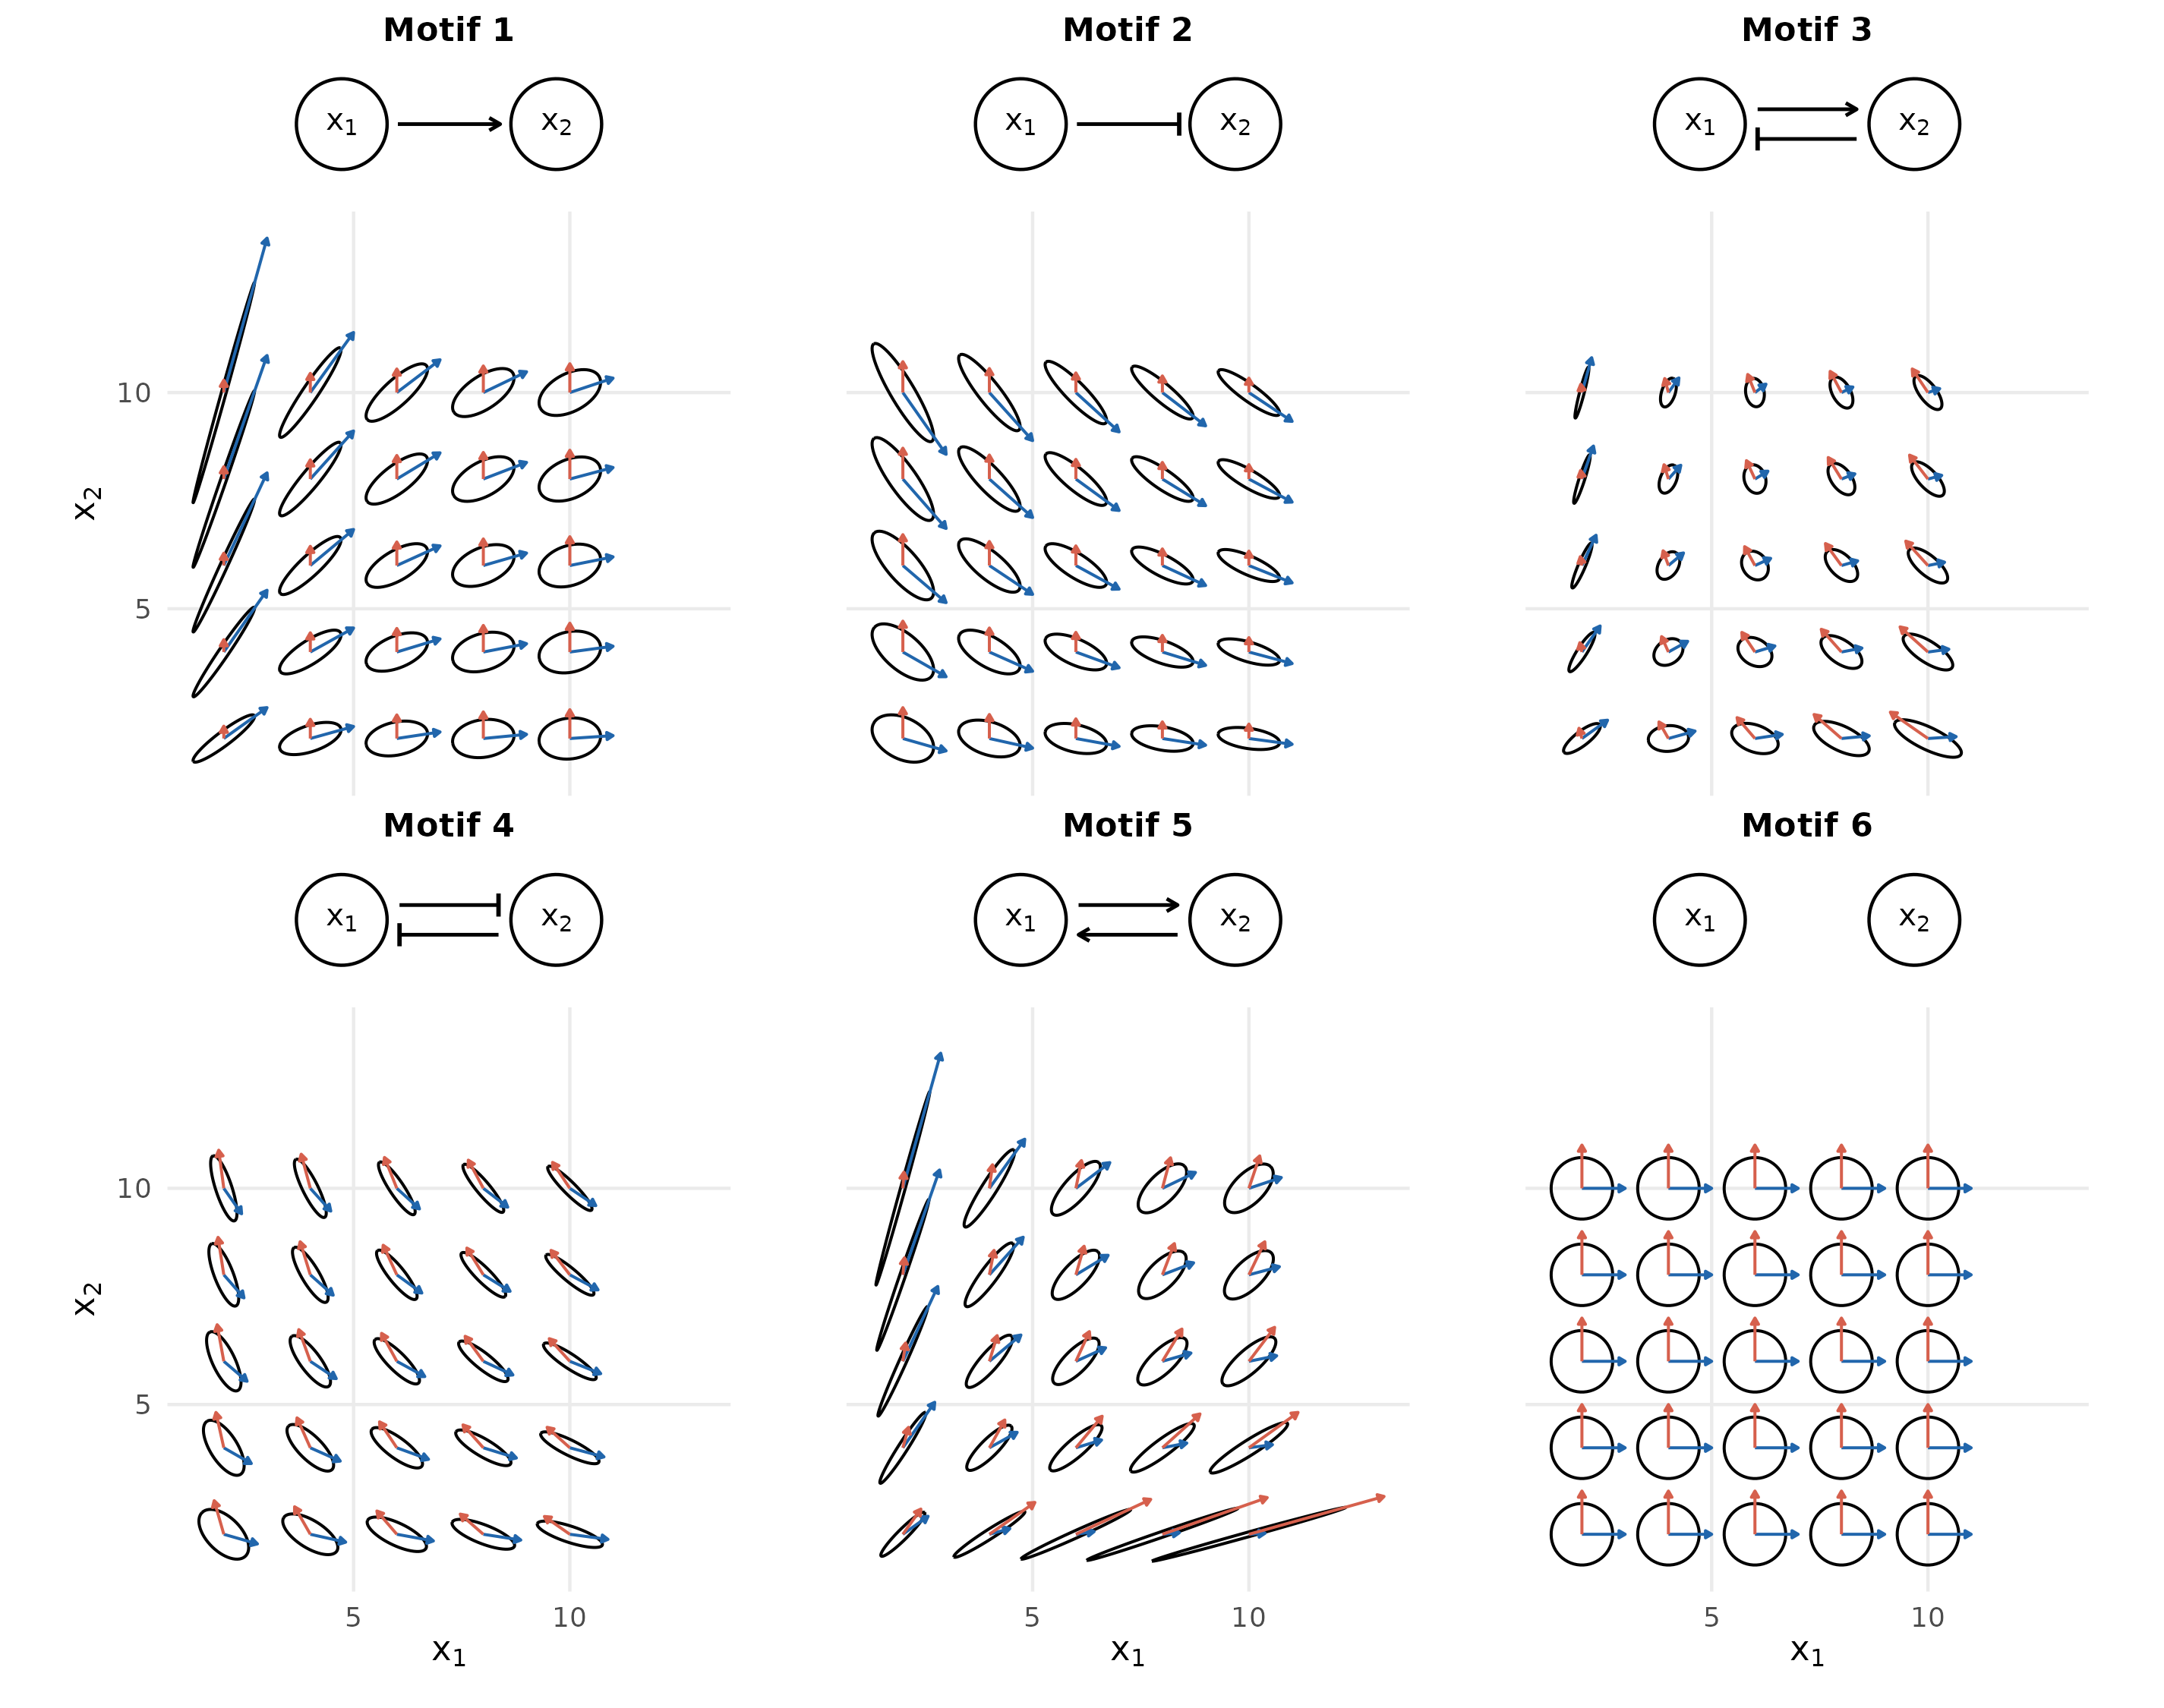
\includegraphics[width=0.65\textheight]{src/figures/fig2.png}
    \caption{\textbf{Gene regulatory motifs and M-matrices.} Gene regulatory motifs between genes $x_1$ and $x_2$, controlled by activation rates $\alpha_1$ and $\alpha_2$, rate of decay $\gamma$, and a parameter $\theta$ that determines the sensitivity of the regulatory response (full equations given in \nameref{methods}). Each motif induces a tensor field of diploid M-matrices ($\mathbf{M} = 2\mu\sigma^2 \mathbf{S}\mathbf{S}^\top$) over different points in phenotype space, shown as 95\% confidence ellipses with axes magnified by a factor of 26 (per-allele mutation rate $\mu=0.025$, standard deviation $\sigma=0.05$). Sensitivity vectors on $\alpha_1$ and $\alpha_2$ are shown in blue and red, respectively (modified from figures 1 and 2 of \cite{hether2014genetic}).}
    \label{fig:fig2}
\end{figure}

\subsection{Evolution under complex genotype-phenotype maps}

We next return to evolutionary simulations to explore how gene regulatory motifs and the M-matrices they induce affect evolutionary outcomes on different adaptive landscapes. As before, we simulate the evolution of populations consisting of 1,000 diploid individuals. The genotype of each individual is the set of $\alpha_1$ and $\alpha_2$ parameters, which now function as the parameters of the regulatory network, and the phenotype is the steady state of gene expression. The complexity of the adaptive landscape is set by the frequency parameter of the Perlin noise, with higher frequencies corresponding to a more complex or rugged adaptive landscape (compare frequencies 0.1 and 0.5 in \FIG[]{fig3}, Supplemental \FIG[]{perlin}).  

First, we employ these simulations to determine how GRN motifs affect evolutionary outcomes and thus, the domains of attraction of different local optima on an adaptive landscape. We ran simulations for each motif from a $41 \times 41$ grid of starting points spread evenly over $x_1, x_2 \in [2, 10]$, in 10 replicates each. At every starting point, a monomorphic diploid sexual population was initialized, and the simulation ran until the population mean converged to a local fitness optimum (\nameref{methods}). 

We find that the underlying gene regulatory motif can significantly alter evolutionary outcomes, both on simple and complex adaptive landscapes (\FIG[]{fig3}). The effect of regulatory motifs shows up as a distortion of the domains of attraction around peaks, where the tendency to produce certain kinds of phenotypes over others has a strong influence on evolutionary outcomes. Importantly, unlike the globally linear genotype-phenotype map studied before, the deformation varies across different regions of the map: it is most pronounced in phenotype regions in which the M-matrices are highly eccentric. Thus the nonlinear genotype-phenotype maps induce a deformation of the domains of attraction that also depends on the location in phenotype space. We see e.g. a stronger deformation of the separatrices in motif 1 in the top left corner of the phenotype space, where M-matrices become strongly eccentric. The same can be observed for motif 2 comparing the phenotype region in the bottom left, where M-matrices are nearly unbiased, to the rest of the phenotype space. The deformation of the separatrices leads populations with different motifs to settle on different optima despite starting from the same origin. The results for all six motifs across both the simple and complex adaptive landscapes are shown in Supplemental \FIG[]{figS1}, \FIG[]{figS2}.

We can further characterize these motif-dependent deformations analytically. Indeed, in the specific scenario where populations begin monomorphic and M-matrices can be uniquely identified at every point in phenotype space, we can use a modified version of the Lande equation \parencite{lande1979quantitative} to determine the separatrices between alternative evolutionary outcomes. Specifically, we assume that for each point in phenotype space, $\mathbf{M}\propto \mathbf{G}$, and that phenotypic variation is small relative to the scale of the adaptive landscape, such that $\bar{W}\approx W(\bar{z})$. The adaptive landscape then defines a selection-gradient field that is transformed by the phenotype-dependent genetic covariance tensor field $\mathbf{G}(x_1,x_2)$, yielding a vector field of evolutionary responses on which separatrices can be determined. Since the G-matrices are nonsingular, critical points of the adaptive landscape are preserved, such that local optima remain stable, and separatrices of different motifs cross at the saddle points. The thus-derived separatrices agree well with those observed in simulation (cf. black and white lines in Supplemental \FIG[]{figS1}, \FIG[]{figS2}). 

\begin{figure}[p]
    \centering
    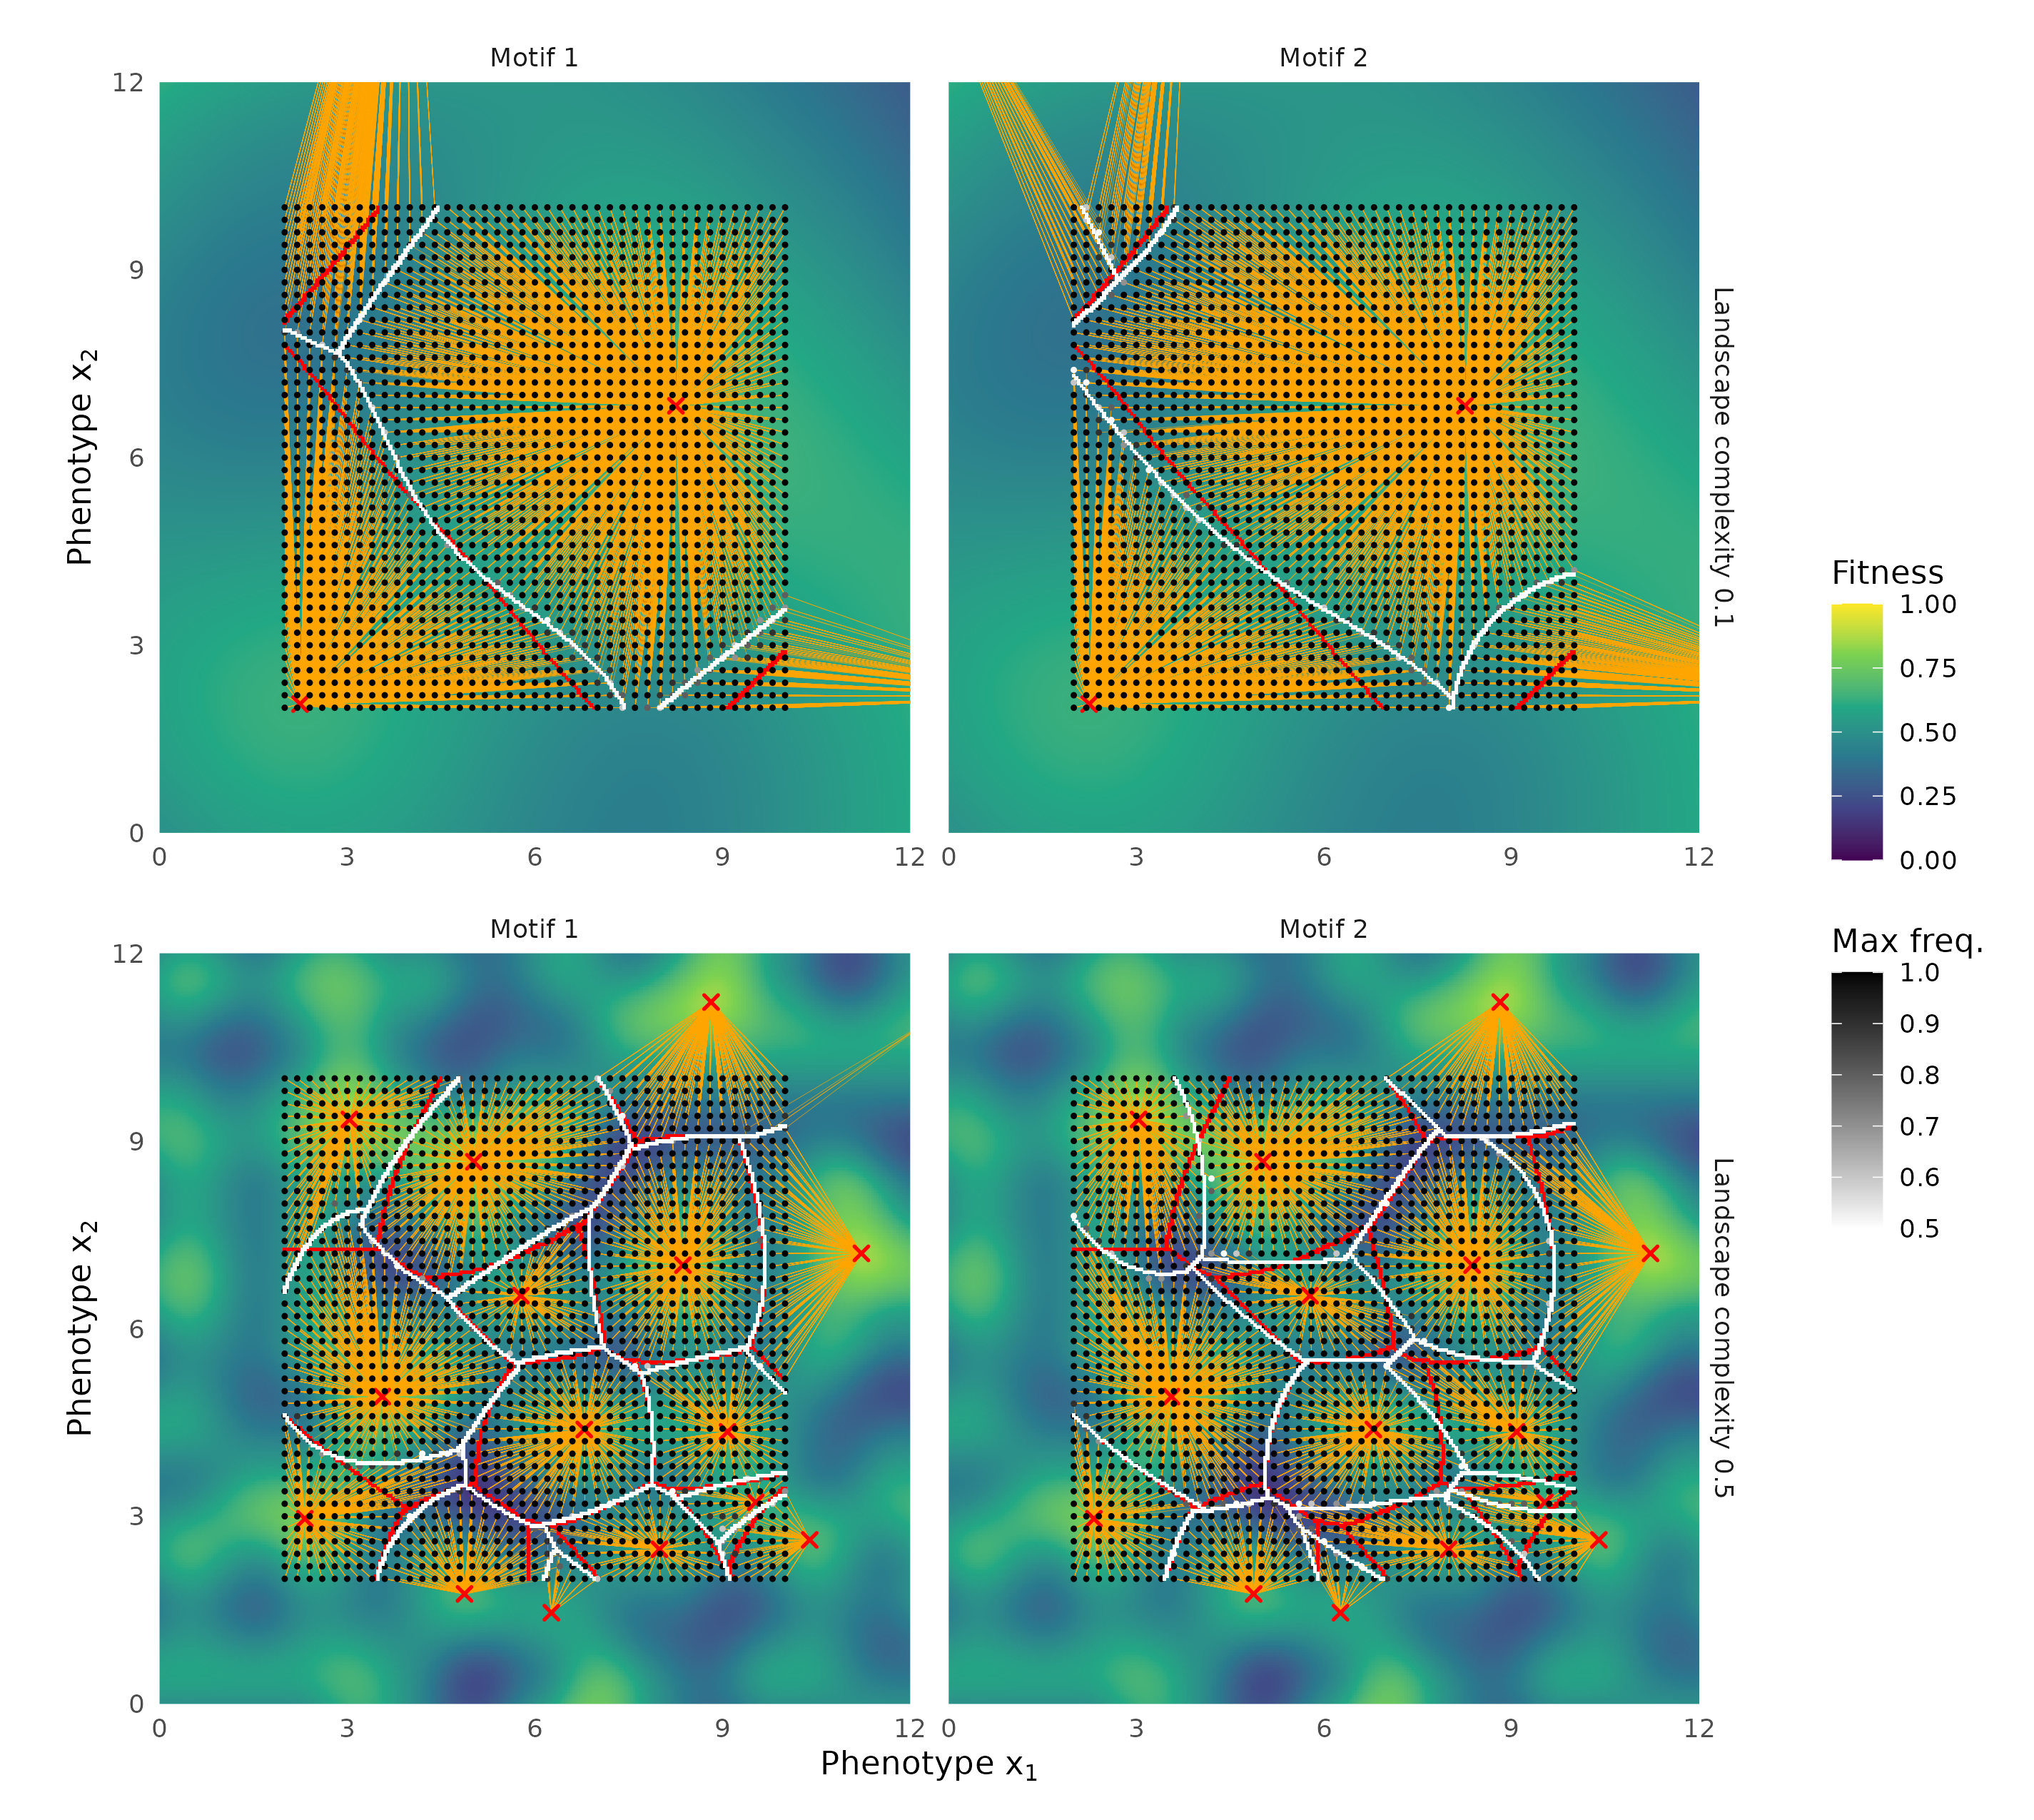
\includegraphics[
        width=\linewidth,
        height=0.9\textheight,
        keepaspectratio
    ]{src/figures/fig3.png}
    \caption{\textbf{Evolutionary outcomes on two adaptive landscapes of different complexity.} We explore a $41 \times 41$ grid of starting points, spaced evenly over $x_1, x_2 \in [2, 10]$, and simulate the evolution of 10 diploid sexual replicates over up to 10,000 generations, or until a local fitness optimum has been reached, for motifs 1 (left) and 2 (right). Local optima are highlighted by a red mark, and starting points and outcomes are connected by orange edges. Starting points are colored according to the frequency of the most frequent evolutionary outcome. Regions of ambiguity, shown in shades of grey, arise when replicate populations originating from the same starting point reach different local optima due to stochastic differences. The observed domains of attraction for each motif as inferred by SVM are delineated in white, and the domains of attraction for motif 6 are shown in red, providing a comparison with a GRN without developmental bias. The 10-fold cross-validated classification accuracy of the SVM for motifs 1, 2, and 6 was 99.0\%, 98.8\%, and 98.3\% on the simple landscape and 97.8\%, 97.3\%, and 97.8\% on the complex landscape. The adaptive landscapes were generated as Perlin noise with a frequency of 0.1 (seed 1234, top row) and 0.5 (seed 1245, bottom row). }
    \label{fig:fig3}
\end{figure}



\subsection{Adaptive landscape complexity}

Next, we systematically survey how the complexity of the adaptive landscape affects evolutionary outcomes between different gene regulatory motifs. Across four Perlin frequencies (0.3, 0.6, 1.2, and 1.8) with 20 randomly generated landscapes per frequency, we simulate each motif from a $25 \times 25$ grid of starting points over $x_1, x_2 \in [2, 10]$ (one replicate per starting point) and quantify how often populations with different regulatory motifs but the same point of origin evolve towards alternative local optima, a measure we term `outcome mismatch'. More specifically, retaining starting points where all six motifs converged, we compare the evolutionary outcomes observed under a given motif with the evolutionary outcomes observed under motif 6, the GRN with a stable, spherical M-matrix across phenotype space (\FIG[]{fig4}). 

We see that outcome mismatch increases consistently as the adaptive landscape becomes more rugged, rising from mean values of 0.09--0.14 at frequency 0.3 to 0.29--0.38 at frequency 1.8. The variance of outcome mismatch across landscapes is initially larger (SD 0.04--0.05 at frequency 0.3) and decreases as landscapes become more rugged (SD 0.02--0.03 at frequency 1.8). This is because adaptive landscapes sampled from low-frequency noise are more variable with regard to the number and arrangement of evolutionary optima than landscapes sampled from high-frequency noise.
The pairwise comparison of evolutionary outcomes across all six network motifs shows that motif 5 is most dissimilar from the other motifs, but shares most evolutionary outcomes with motif 1 (\FIG[B]{fig4}), with which it has activating gene interactions in common and nearly identical M-matrices over half the phenotype space (\FIG[]{fig2}). Likewise, motifs 2 and 4, which share the same inhibitory interaction $x_1 \dashv x_2$, have most outcomes in common with each other. Outcome mismatch is sensitive to the distribution of mutations, which we here set to $\sigma=0.2$. Under default conditions ($\sigma=0.05$, 10 landscapes per frequency on a $21 \times 21$ grid), the overall pattern remains the same, with lower mean outcome mismatch reaching 0.09--0.16 (approximately 0.15 across motifs 2, 4, and 5) at the highest level of landscape frequency.

We further investigated how well the leading eigenvector of the M-matrix is aligned with the direction of evolutionary divergence, defined here as the direction from a population's starting point to the local optimum it ultimately reaches (\FIG[]{fig5}). For motif 6, $\mathbf{M}$ is exactly isotropic, so the leading eigenvector returned numerically is an arbitrary coordinate axis and the uniform angle distribution between 0\degree and 90\degree (median 44.1\degree--45.5\degree) reflects the isotropic distribution of divergence directions across landscapes. For the other five motifs, alignment between evolutionary divergence and $M_{\max}$ is modest when landscape complexity is low (medians 34.3\degree--39.2\degree at frequency 0.3). As the adaptive landscape becomes more rugged, however, the direction of evolutionary divergence becomes increasingly aligned with the leading eigenvector (medians dropping to 22.0\degree--35.7\degree at frequency 1.8), demonstrating that developmental bias has an increasing influence on evolutionary outcomes the more rugged the adaptive landscape becomes. Among the motifs, we observe a consistent pattern in which alignment is strongest in motif 5 (median 22.0\degree at frequency 1.8), followed by motif 4 (25.7\degree), motifs 1 and 2 (26.8\degree), and weakest in motif 3 (35.7\degree), following the eccentricity of the M-matrices these motifs exhibit in the sampled phenotype space.
%%


\begin{figure}
    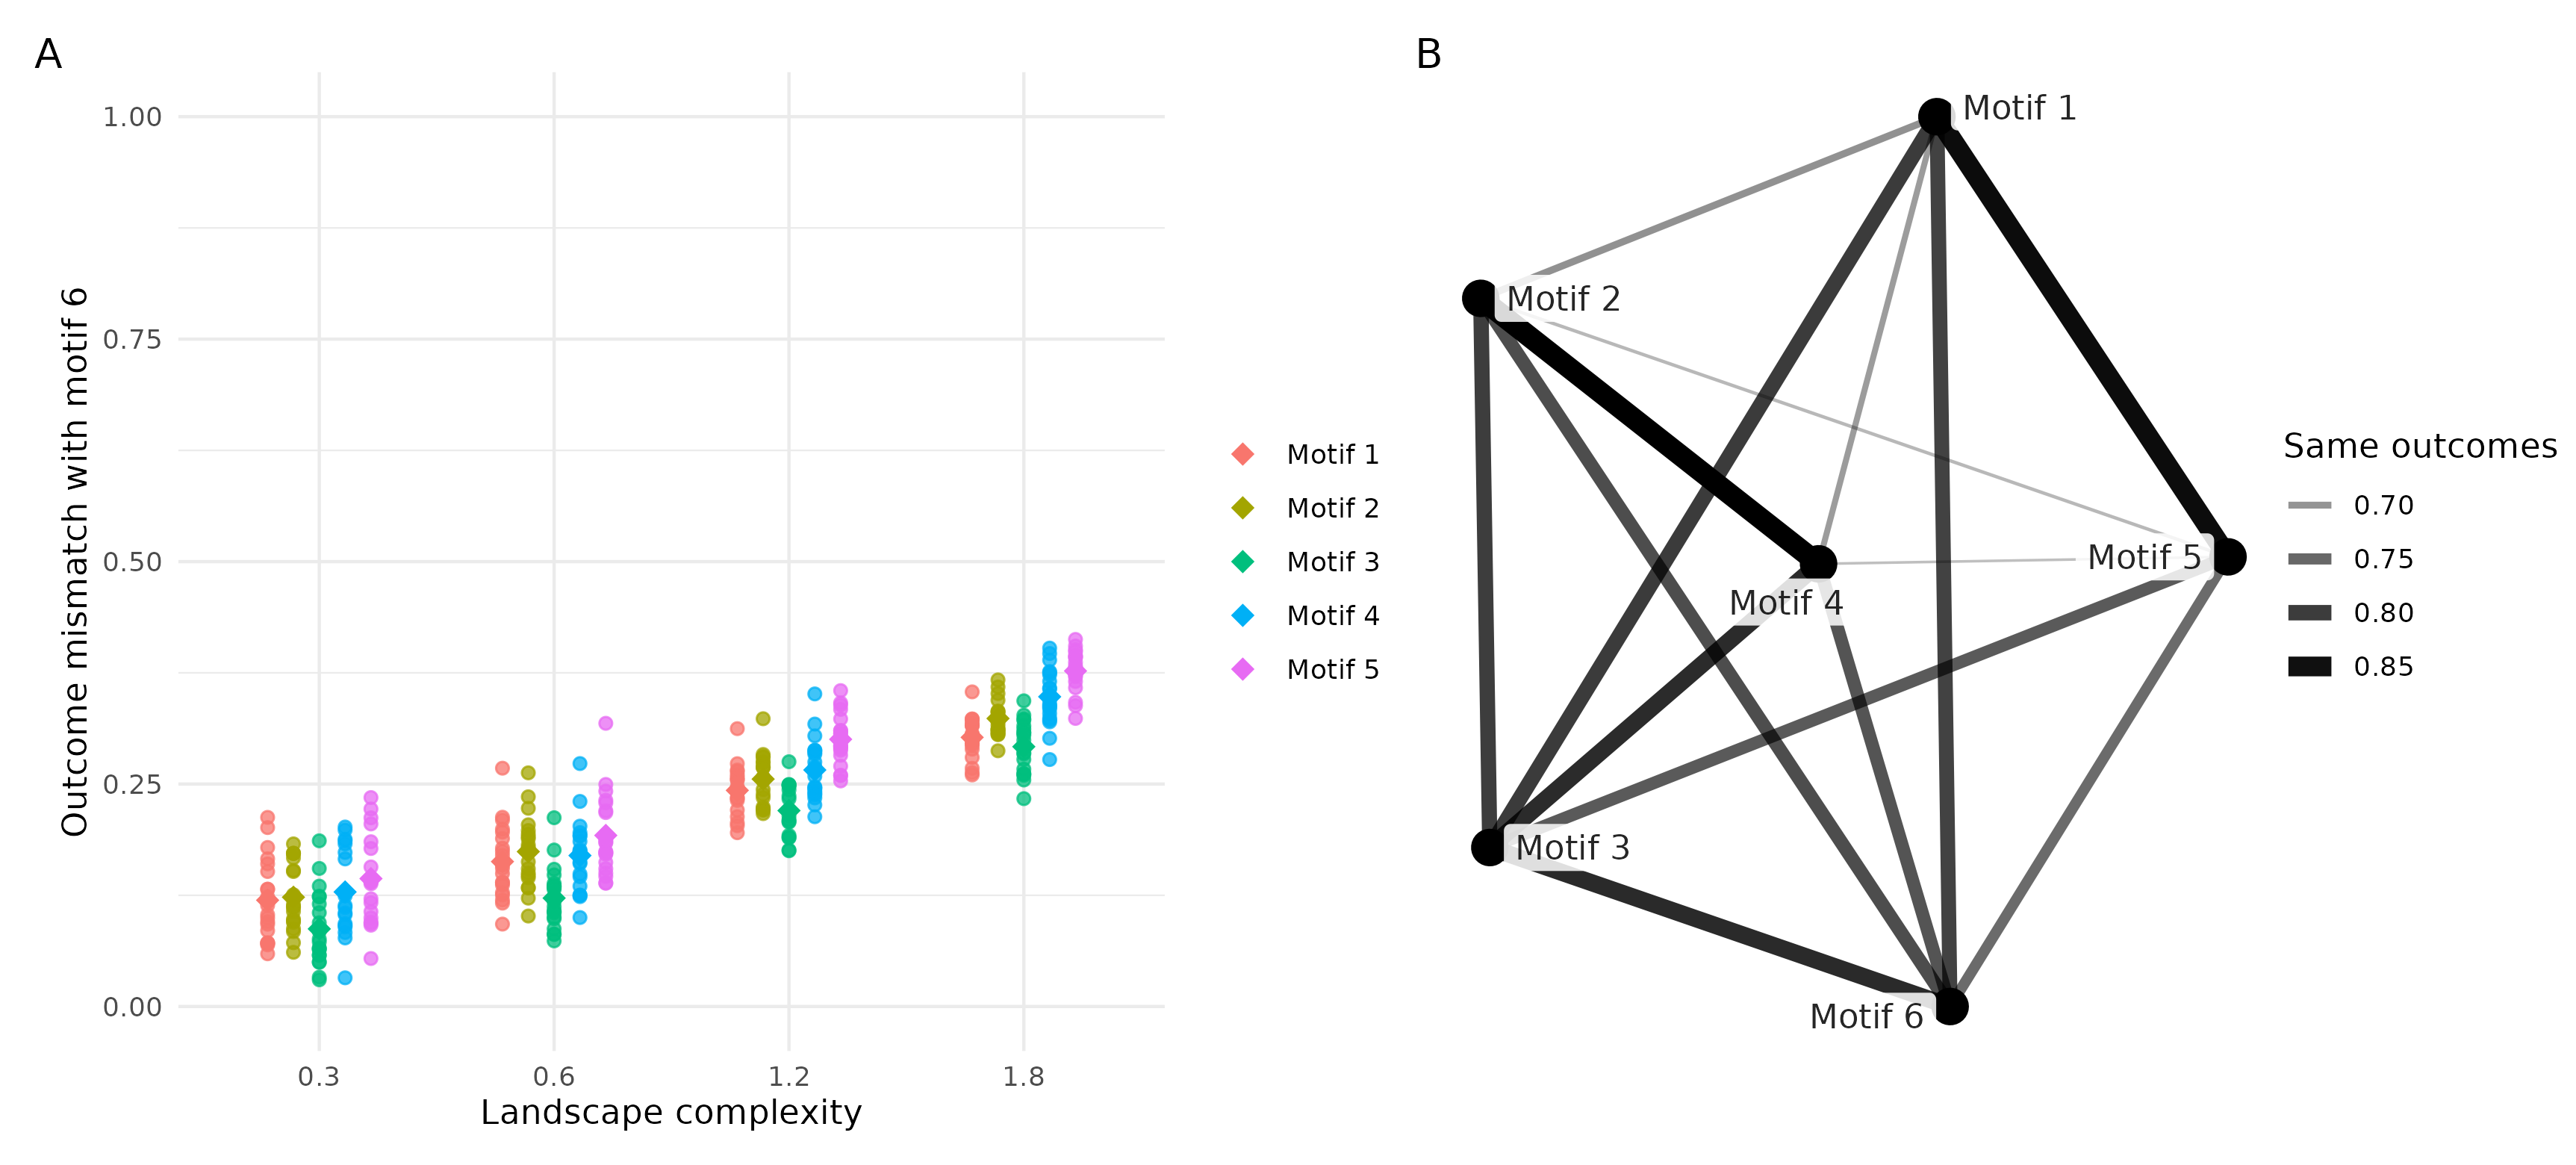
\includegraphics[width=0.65\textheight]{src/figures/fig4.png}
    \caption{\textbf{Mismatch of evolutionary outcomes between different GRNs in dependence of landscape complexity. (A)} Outcome mismatch with motif 6 across 20 random landscapes per Perlin frequency (circles: individual landscapes; diamonds: frequency means; $25 \times 25$ starting grid, $\sigma=0.2$). \textbf{(B)} Pairwise proportion of identical evolutionary outcomes between GRN motifs, pooled across frequencies and landscapes. }
    \label{fig:fig4}
\end{figure}

\begin{figure}
    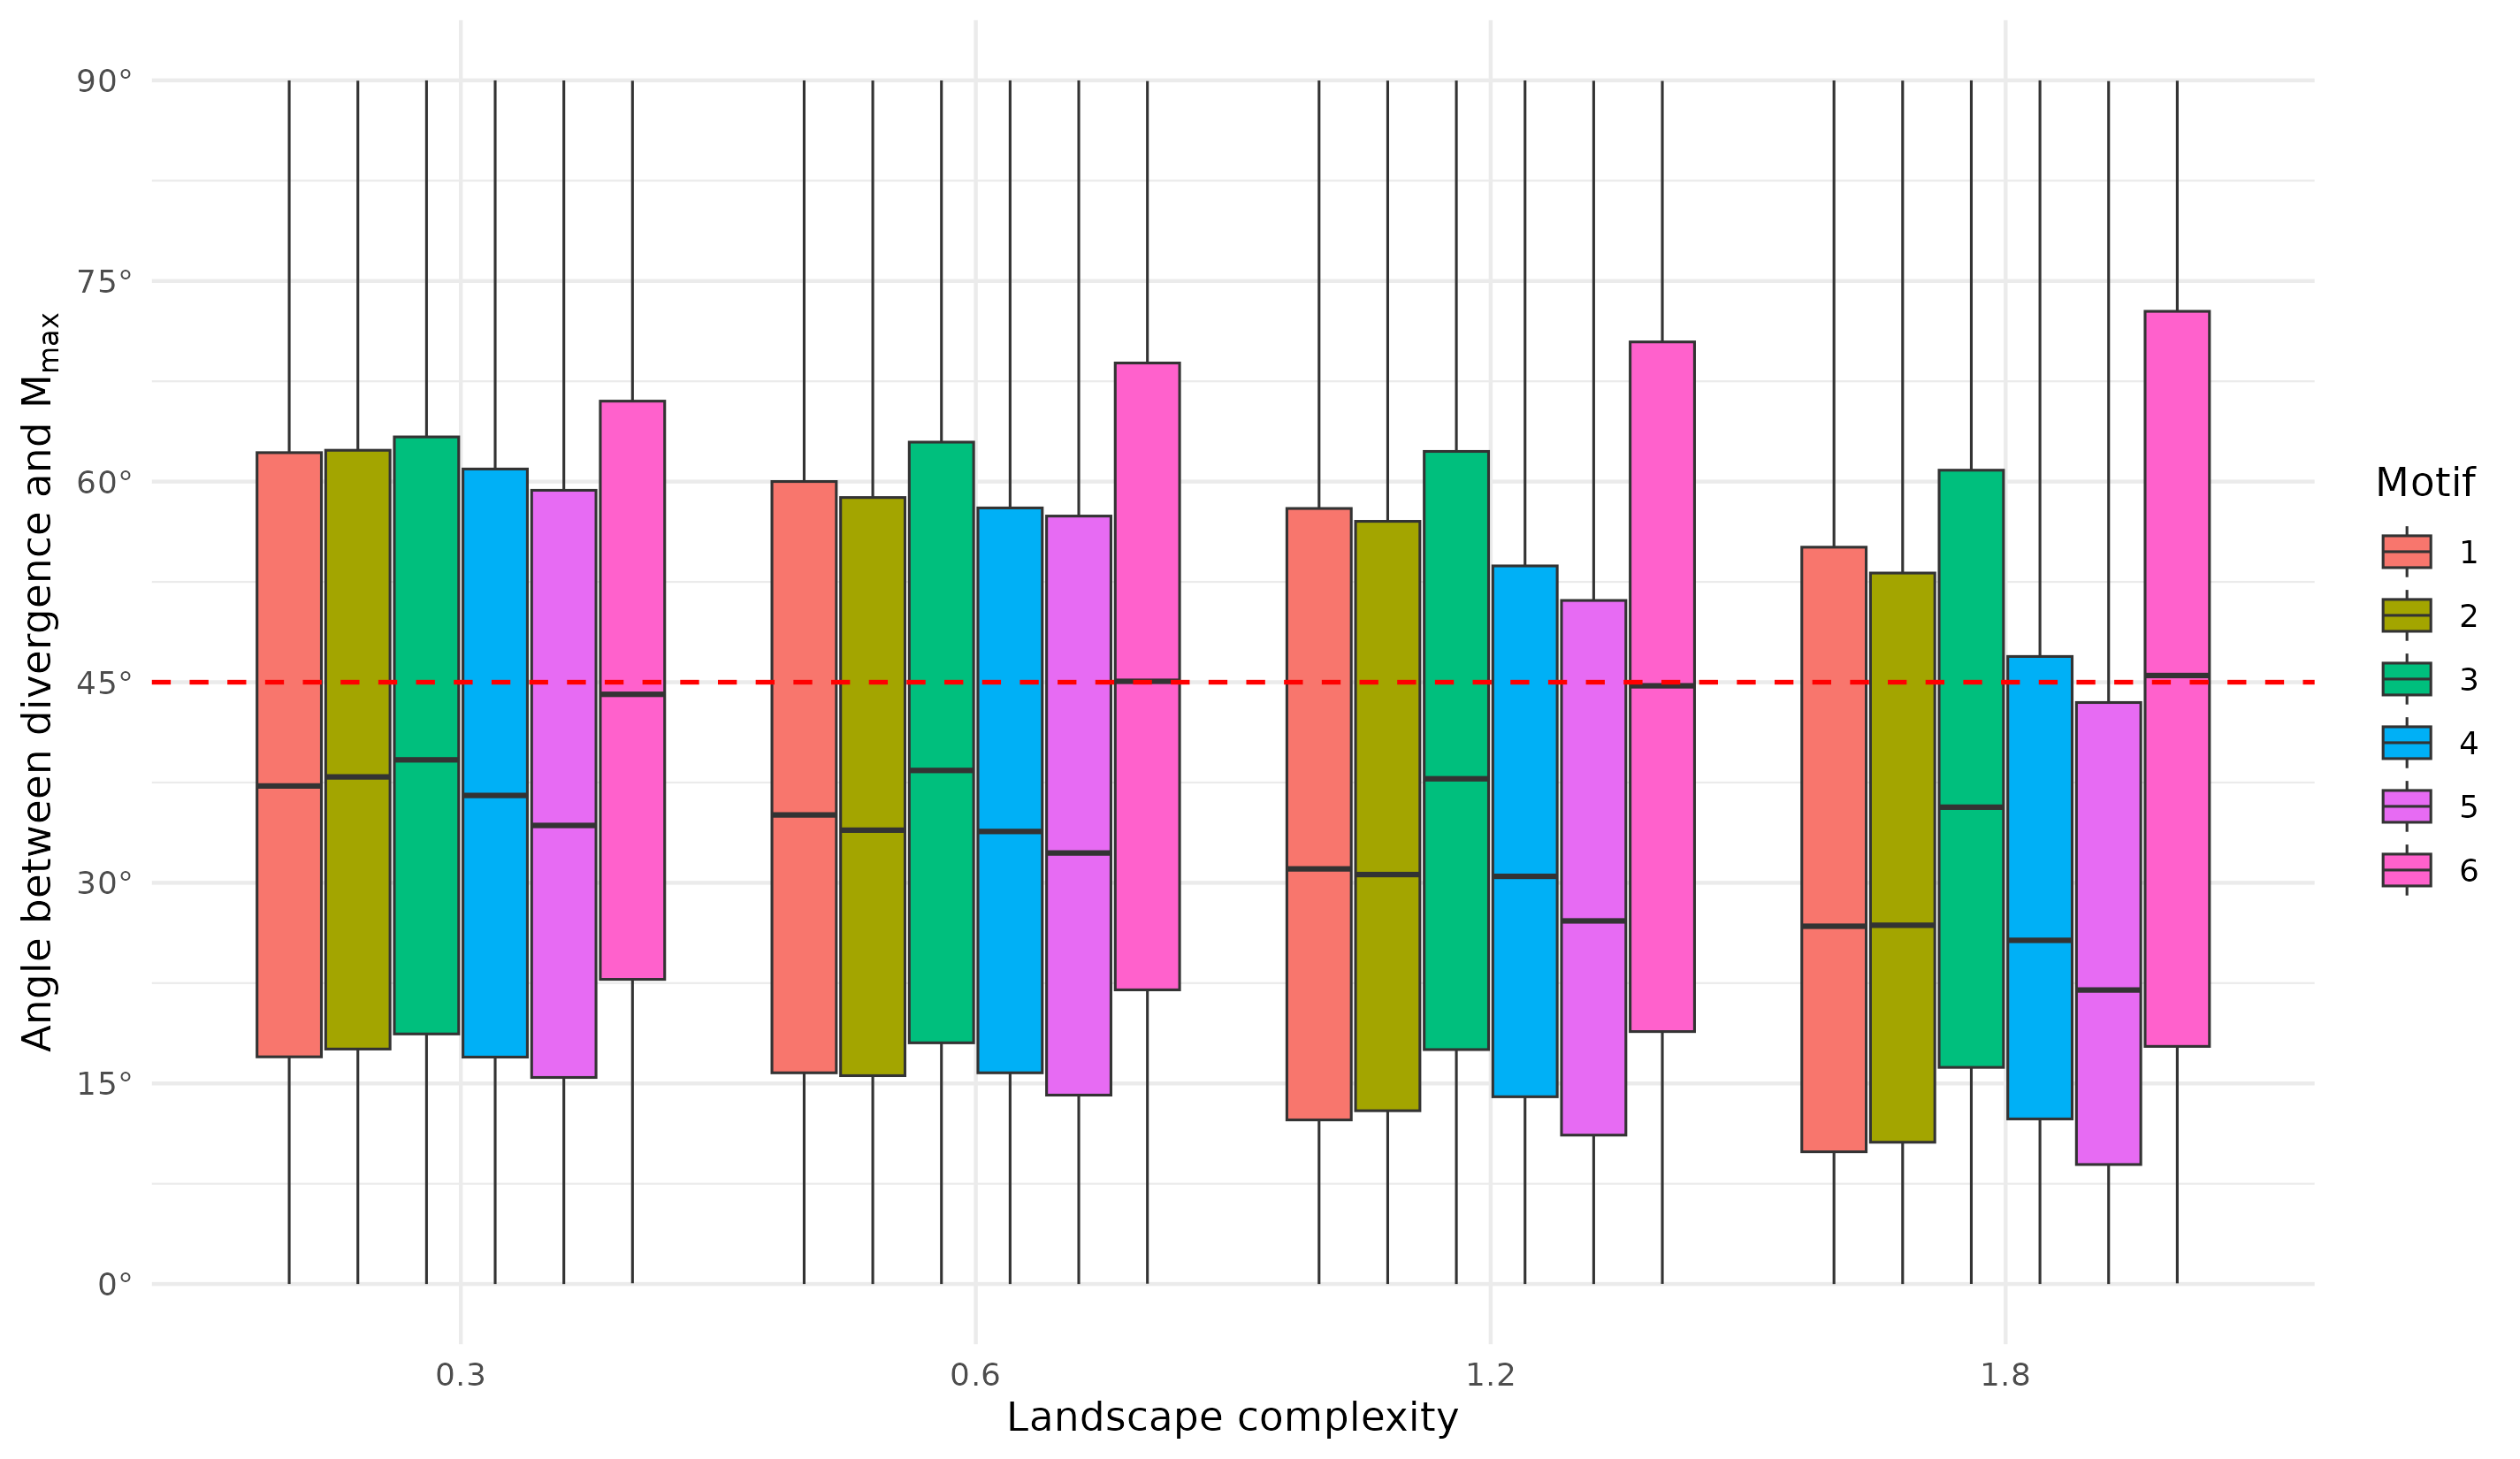
\includegraphics[width=\linewidth]{src/figures/fig5.png}
    \caption{\textbf{Alignment of evolutionary divergence and M-matrix in dependence of landscape complexity.} The angle between the divergence vector (from starting phenotype to reached optimum) and the dominant eigenvector $M_{\max}$ of the M-matrix at the evolutionary end point becomes increasingly aligned as landscapes become more complex. For isotropic M-matrices (motif 6), the numerical eigenvector is arbitrary and angles are uniformly distributed between $0^{\circ}$ and $90^{\circ}$ around a median of $45^{\circ}$ (dashed red line). As landscape complexity increases, the direction of evolutionary divergence and $M_{\max}$ become increasingly aligned for all regulated motifs. Simulations as in \FIG[]{fig4}. }
    \label{fig:fig5}
\end{figure}

\subsection{Evolutionary trajectories}

We have previously shown that regulatory motifs can affect evolutionary outcomes through the distortion of the distribution of mutations. Here, we demonstrate the special case that even populations starting with nearly identical local M-matrices can diverge along their evolutionary trajectories as the genotype-phenotype map changes over phenotype space.
We illustrate this using motifs 1 and 5, which have very similar M-matrices in the top left region of phenotype space (\FIG[]{fig2}). More specifically, at $(x_1, x_2) = (1.0, 4.0)$, the diploid M-matrices of motifs 1 and 5 have nearly identical eccentricity and direction of dominant eigenvectors (eccentricity 0.99991 vs. 0.99986; angle between dominant eigenvector and the $x_1$-axis 73.34\degree vs. 73.40\degree, \FIG[C]{fig6}). Their determinants are also comparable ($4.34 \times 10^{-10}$ vs. $2.97 \times 10^{-10}$), indicating that the matrices differ primarily in scale, with $\mathbf{M}_1$ having a $\sim$46\% larger determinant. 

From this common starting point, we initialize 10 replicate diploid sexual populations of 10,000 individuals per motif on a twin-peak adaptive landscape constructed as the smooth maximum of two shifted, squared frequency-0.05 Perlin layers (\nameref{methods}), which holds two adjacent peaks at $(7.61, 8.21)$ and $(8.45, 9.05)$. We simulated evolution over 6,000 generations, long enough for all replicates to reach their respective optima, and tracked mean phenotypes, M-matrices, and G-matrices every 50 generations (\FIG[]{fig6}). We estimated the additive genetic covariance matrix ($\mathbf{G}$) via mid-parent--offspring regression by independently sampling 5,000 random female--male pairs from the population at each recorded generation, irrespective of fitness, generating one recombinant offspring per pair, and computing $\hat{\mathbf{G}} = \mathrm{Cov}(\mathbf{z}_O, \bar{\mathbf{z}}_P) + \mathrm{Cov}(\mathbf{z}_O, \bar{\mathbf{z}}_P)^\top$.

Both motifs initially evolved together along their shared, strongly eccentric axis of mutational variation before turning along the ridge toward the twin peaks (\FIG[A]{fig6}). As the populations moved into higher $x_1$ and $x_2$ values, however, their M-matrices diverged: motif 1's M-matrix decreased in eccentricity (to 0.86) and rotated to a shallower angle (30.4\degree), whereas motif 5 retained higher eccentricity (0.90) and a steeper positive covariance (45.1\degree; \FIG[C]{fig6}). Consequently, the trajectories branched reliably across replicates: 9 of 10 motif 1 replicates converged on the upper-right peak at $(8.45, 9.05)$, whereas all 10 of 10 motif 5 replicates turned onto the lower-left peak at $(7.61, 8.21)$. Throughout directional evolution, the parent--offspring G-matrix tracked the orientation and eccentricity of the M-matrix with substantial stochasticity (\FIG[B, C]{fig6}). Once motif 1 settled at its optimum, stabilizing selection reduced the eccentricity of $\mathbf{G}$ below that of $\mathbf{M}$. Together, these results show that differences in the underlying genotype-phenotype map can lead to divergent evolution of local developmental bias and, consequently, to reliably different evolutionary trajectories and outcomes, even when initial local M-matrices are nearly identical.

\begin{figure}
    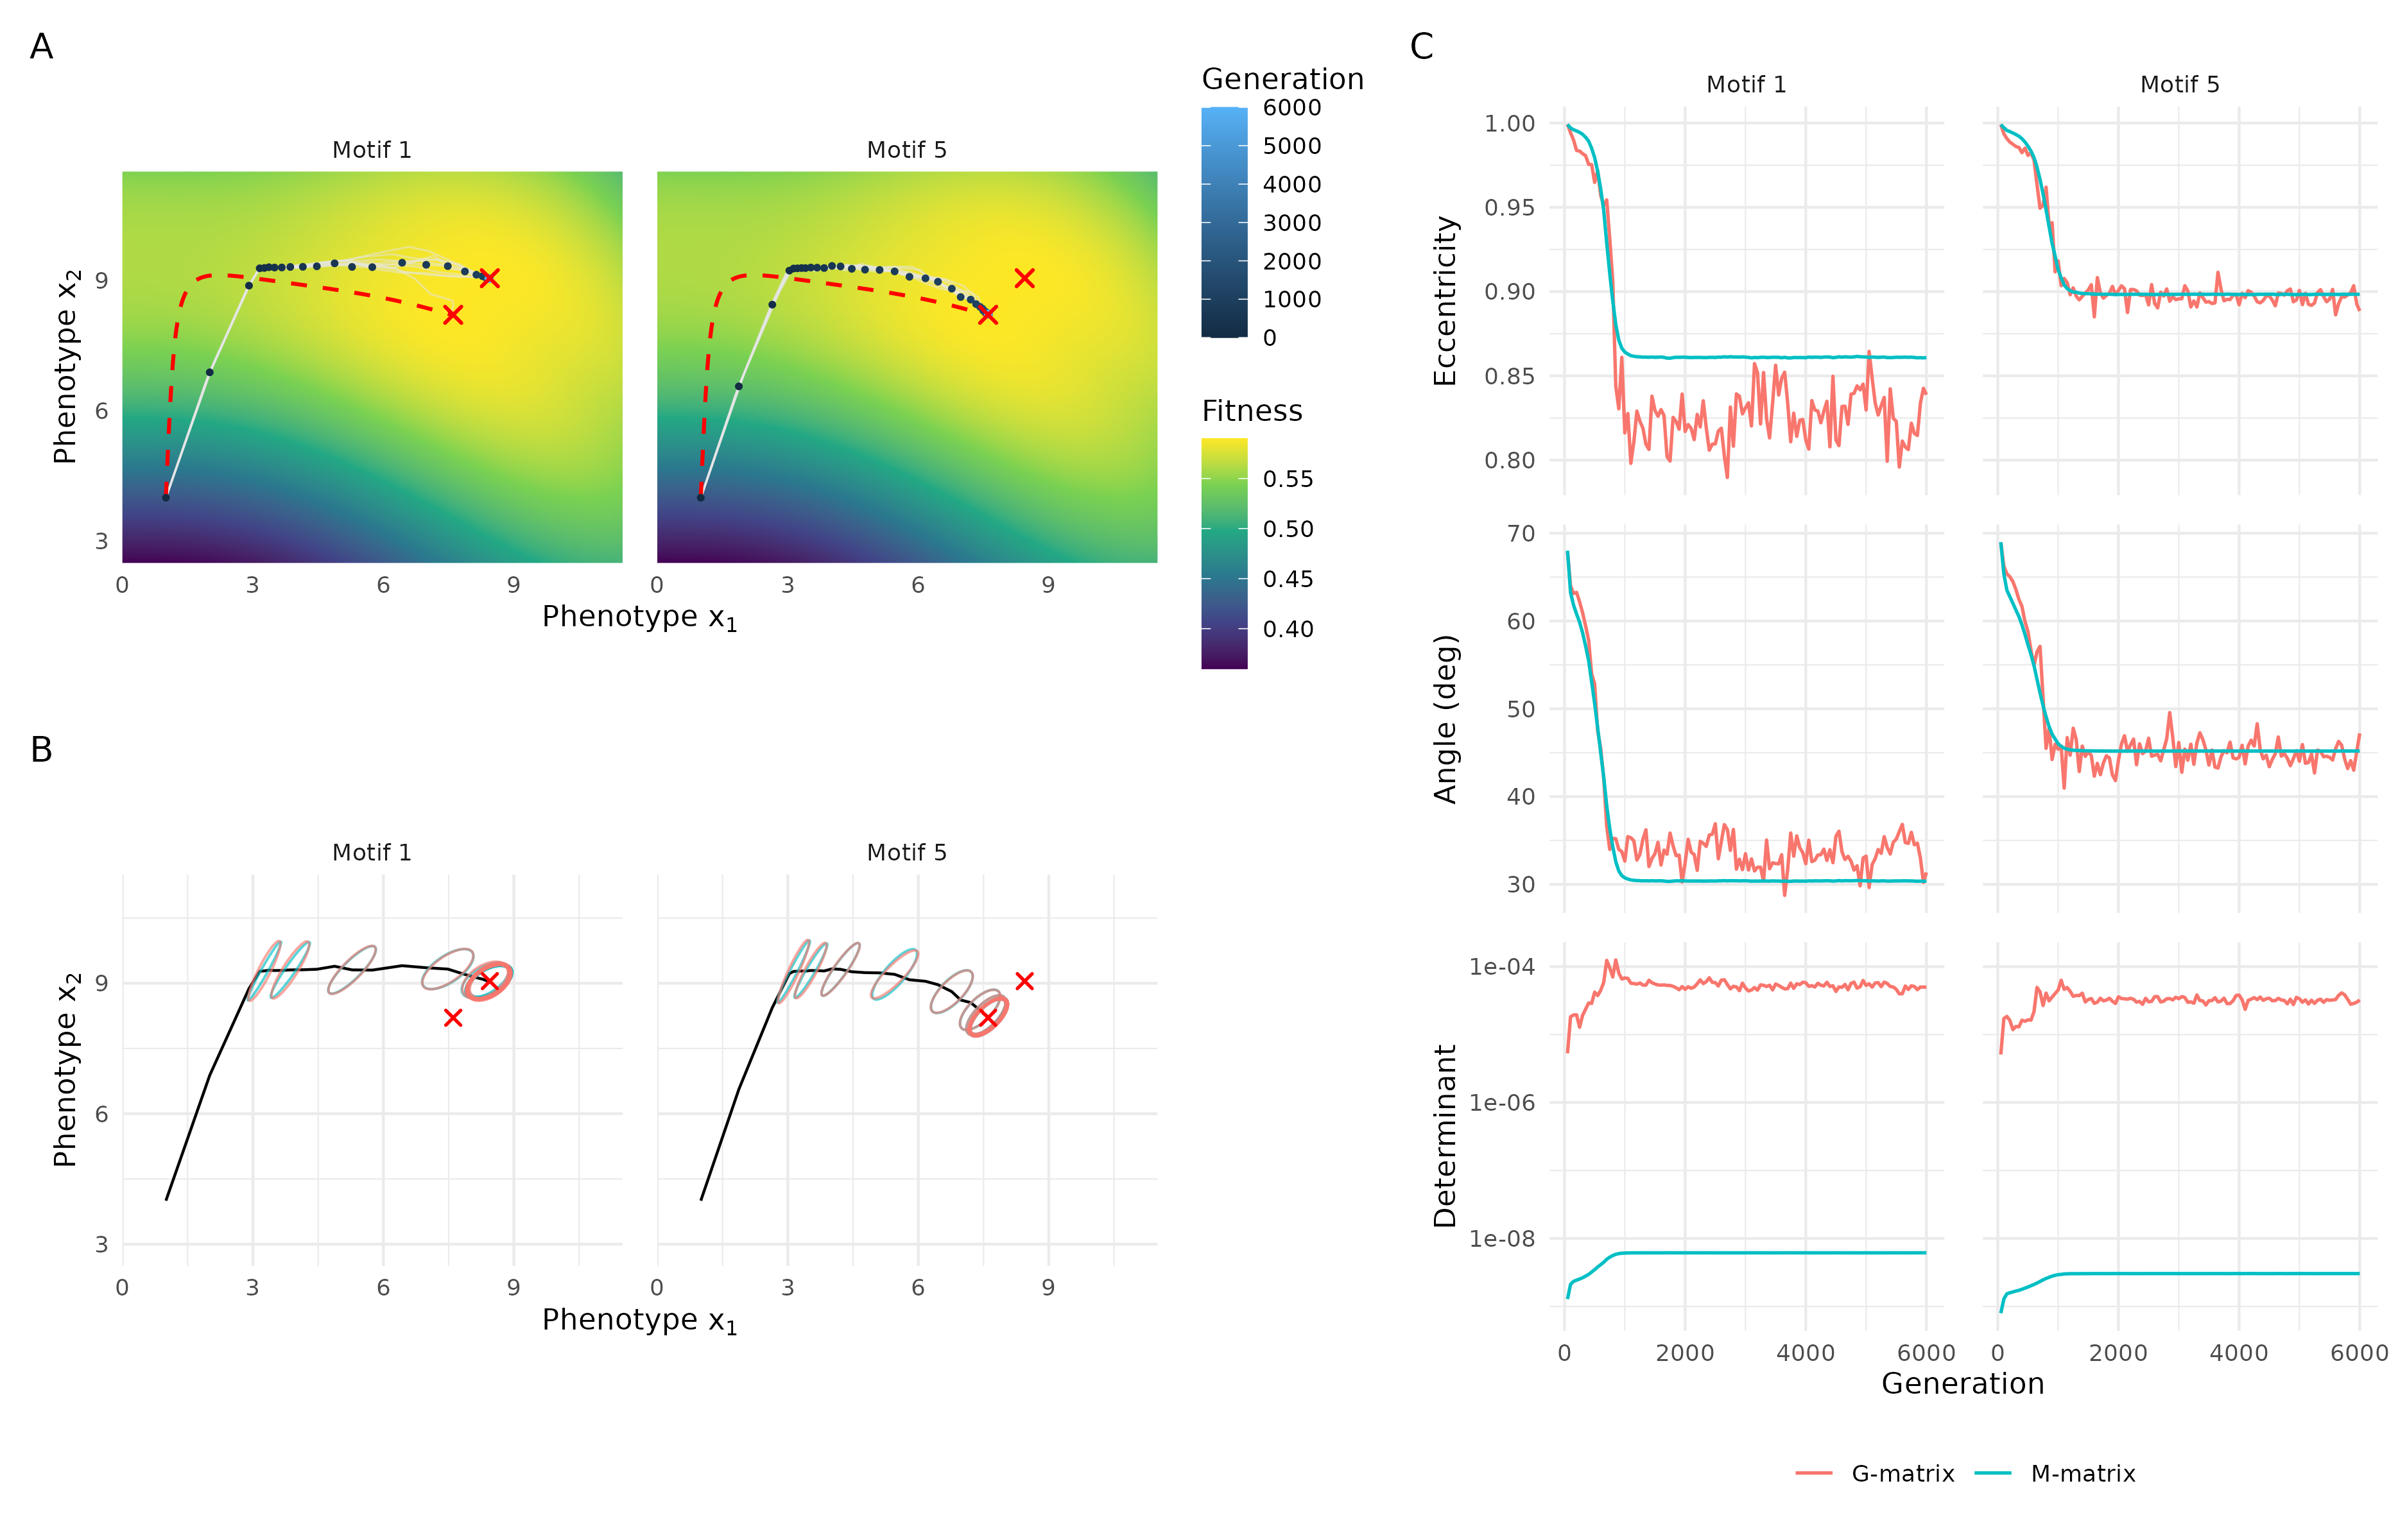
\includegraphics[width=\linewidth]{src/figures/fig6.png}
    \caption{\textbf{Evolutionary trajectories on a twin-peak adaptive landscape.} Ten replicate diploid sexual populations ($N = 10{,}000$) per motif are initialized at $(1.0, 4.0)$ and evolve over 6,000 generations on a smooth-maximum landscape with adjacent peaks at $(7.61, 8.21)$ and $(8.45, 9.05)$ (red crosses). \textbf{(A)} Adaptive landscape and evolutionary trajectories (representative replicate colored dark to bright blue from generation 0 to 6,000; light grey curves show all 10 replicates; dashed red line shows the path of steepest ascent). Nine of 10 motif 1 replicates reach $(8.45, 9.05)$ and 10 of 10 motif 5 replicates reach $(7.61, 8.21)$. \textbf{(B)} Representative trajectories of mean phenotypes with parent--offspring G-matrices (salmon) and trace-matched M-matrices (teal), plotted every 200 generations as 95\% confidence ellipses with axes magnified by a factor of two. \textbf{(C)} Eccentricity, angle of the dominant eigenvector, and determinant (log scale) of the G-matrix (salmon) and M-matrix (teal) over time. }
    \label{fig:fig6}
\end{figure}


